\documentclass[12pt]{article}
\usepackage[a4paper, total={6in, 9in}]{geometry}
\usepackage{graphicx}
\graphicspath{ {./images/output/} }
\usepackage{caption}
\usepackage[english]{babel}
\usepackage{titling}
\usepackage{float}
% \usepackage{amsmath}
% \usepackage{minted}
% \usepackage{multicol}
% \usepackage{array}
% \usepackage{setspace}
% \usepackage{placeins}

% \usepackage{lipsum}

\title{Study of Thyristor Characteristics R, RL Load}
\author{}
\date{}

\pagenumbering{gobble}
\begin{document}
\vspace*{\fill}
\begin{center}

    \emph{Heaven's Light is Our Guide} \\
    \textbf{Rajshahi University of Engineering and Technology} \\

    \begin{figure}[H]
        \centering
        
\includegraphics[scale=.34]{images/RUET_logo.png}
        \label{fig:ruet_logo}
    \end{figure}
    \vspace{5mm}

    \textbf{Course Code}\\
    ECE 3206\\
    \vspace{3mm}
    \textbf{Course Title}\\
    Industrial Electronics Sessional

    \vspace{5mm}
    \textbf{Experiment Date:} {January 13, 2025},\\
    \textbf{Submission Date:} {February 10, 2025}\\

    \vspace{5mm}
    \textbf{Lab Report 3: \\
        Study of Thyristor Characteristics R, RL Load}

    \vspace{15mm}

    \begin{tabular}{c|c}
        \textbf{Submitted to} & \textbf{Submitted by} \\
        Md. Faysal Ahamed     & Md. Tajim An Noor     \\
        Lecturer              & Roll: 2010025         \\
        Dept of ECE, Ruet     &                       \\
    \end{tabular}

\end{center}
\vspace*{\fill}


\pagebreak

\tableofcontents

\pagebreak
\pagenumbering{arabic}
\maketitle

\section*{Theory}
\addcontentsline{toc}{section}{Theory}
In this experiment, the characteristics of a thyristor (SCR) under different load conditions using both DC and AC supplies were investigated using simulation software.

\subsection*{Thyristor Characteristics with DC Supply}
With a DC supply, the thyristor exhibited forward and reverse blocking characteristics. In forward blocking mode, it blocked current until a gate pulse was applied, then conducted until the current fell below the holding current. In reverse blocking mode, it blocked current flow, allowing only a small leakage current until the breakdown voltage was reached \cite{thyristor_characteristics}.

\subsubsection*{R Load}
With a resistive (R) load, the thyristor's behavior is straightforward. When a gate pulse is applied, the thyristor switches to the forward conduction mode, allowing current to pass through the resistive load. The current waveform follows the input voltage waveform, and the thyristor remains on until the current drops below the holding current.

\subsubsection*{RL Load}
With a resistive-inductive (RL) load, the thyristor's behavior is more complex due to the inductance. When a gate pulse is applied, the thyristor switches to the forward conduction mode, and the current through the load increases gradually due to the inductance. The thyristor remains on until the current drops below the holding current, but the inductive load causes the current to continue flowing even after the input voltage drops to zero, resulting in a phase shift between the voltage and current waveforms.

\subsubsection*{Gate Trigger Timing}
The timing of the gate pulse is crucial in controlling the thyristor's conduction. By adjusting the gate trigger timing, the conduction angle of the thyristor can be controlled, which in turn controls the average power delivered to the load. For an R load, the gate pulse timing directly affects the point at which the thyristor starts conducting. For an RL load, the gate pulse timing affects both the conduction angle and the phase shift between the voltage and current waveforms.

\section*{Required Equipments/Software}
\addcontentsline{toc}{section}{Required Equipments/Software}
\begin{itemize}
    \item MATLAB/Simulink
    \item Oscilloscope
    \item AC Voltage Source
    \item Thyristor
    \item Series RLC Branch
    \item Pulse Generator
    \item Measurement Tools
\end{itemize}

\section*{Circuit Diagrams}
\addcontentsline{toc}{section}{Circuit Diagrams}
\begin{figure}[H]
    \centering
    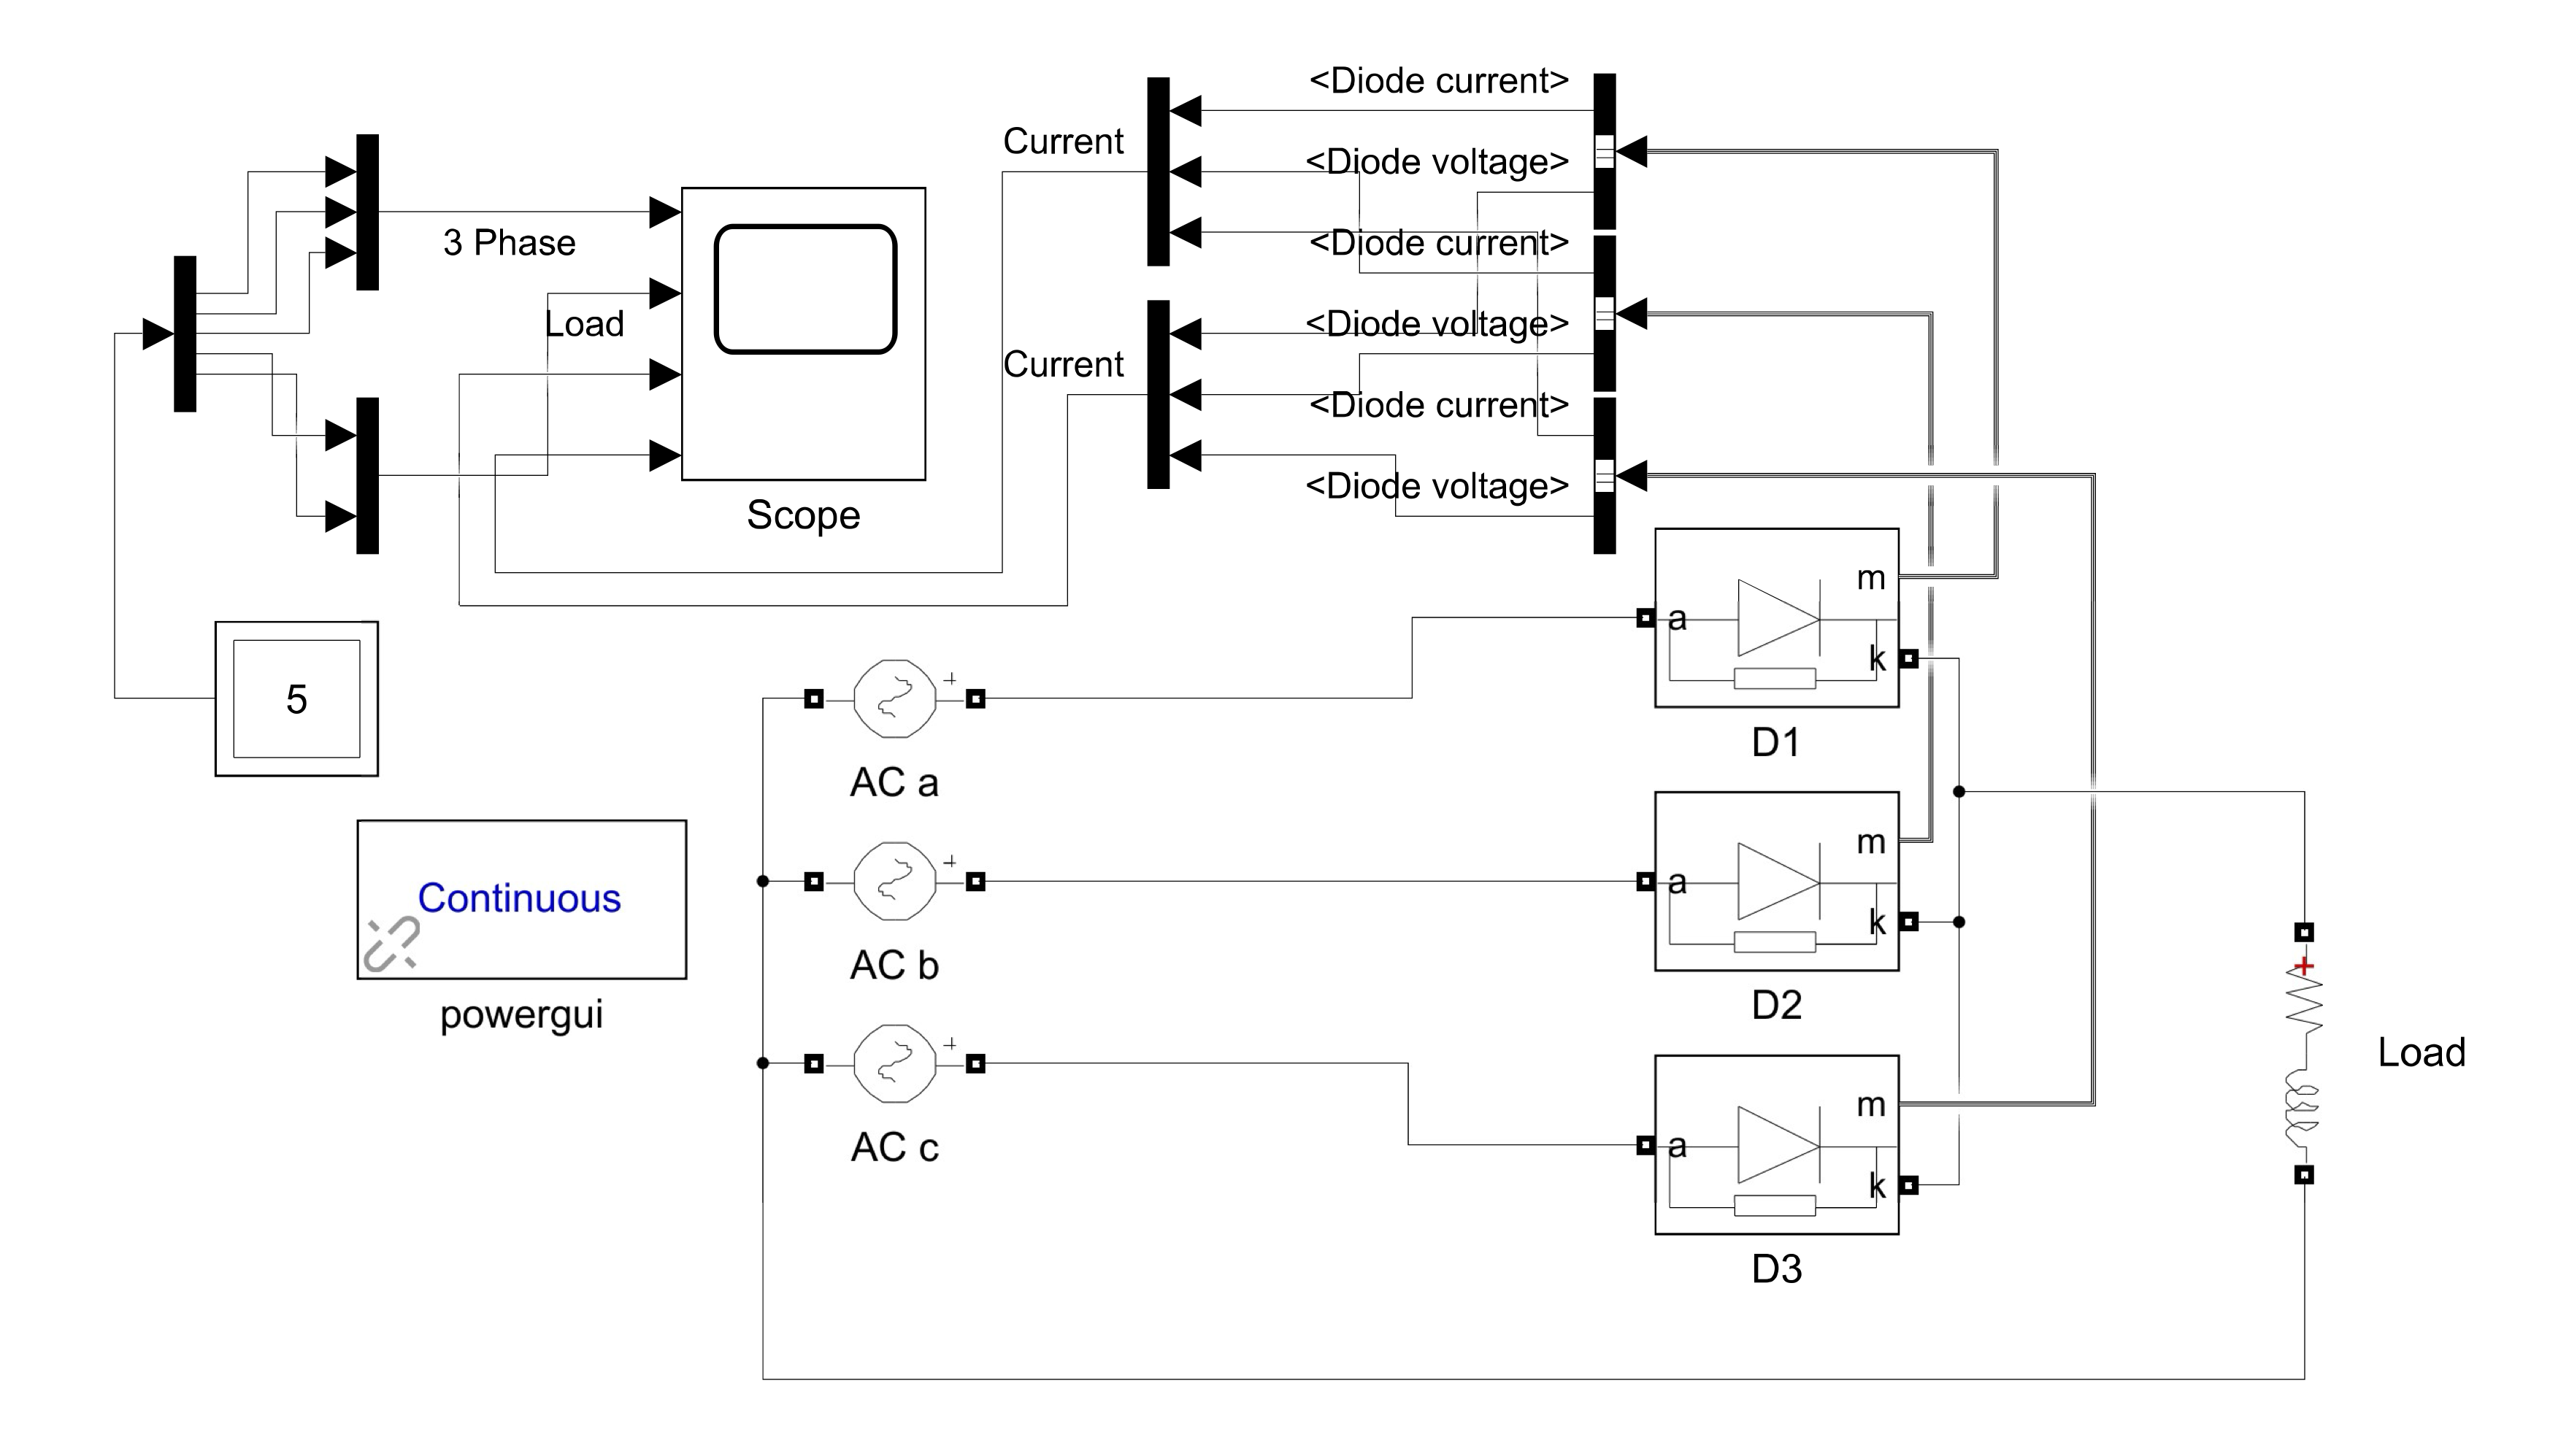
\includegraphics[width=\textwidth]{ckt.png}
    \caption{Diode with Resistive Load}
    \label{fig:dc_r_load}
\end{figure}

\section*{Observations}
\addcontentsline{toc}{section}{Observations}
\begin{itemize}
    \item Observed the input, output, and pulse voltage/current graphs in the oscilloscope.
    \item Four cases were analyzed:
          \begin{itemize}
              \item R Load: With gate voltage delay.
              \item R Load: Without gate voltage delay.
              \item RL Load: With gate voltage delay.
              \item RL Load: Without gate voltage delay.
          \end{itemize}
\end{itemize}

\subsubsection*{Outputs}
\begin{figure}[H]
    \centering
    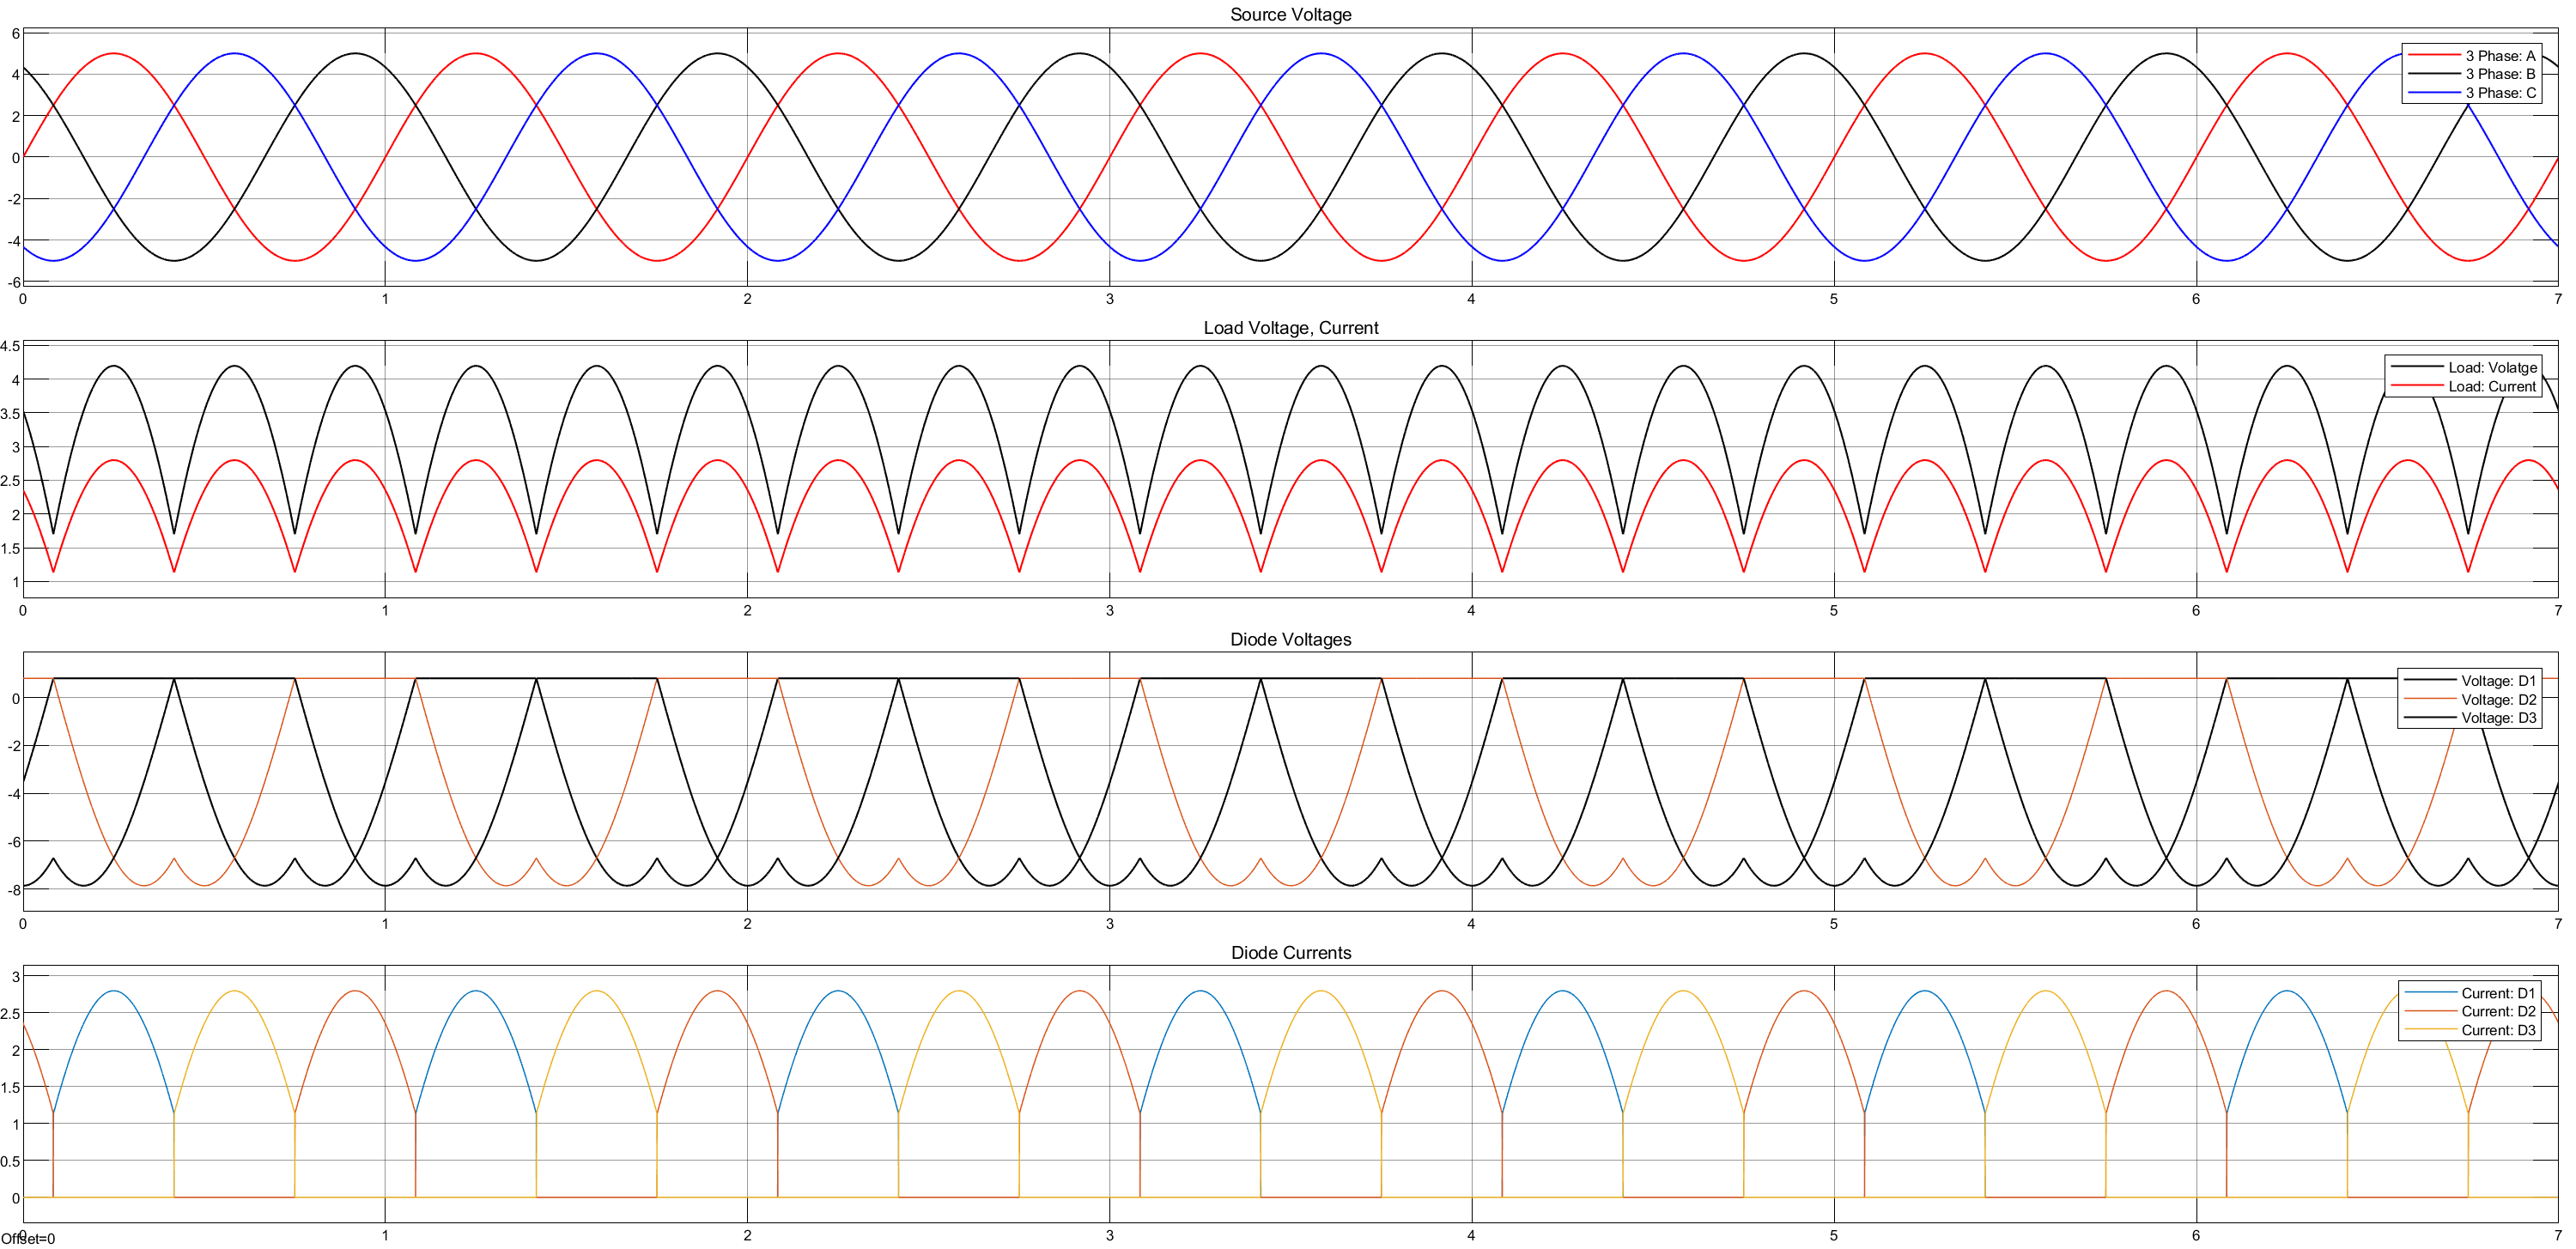
\includegraphics[width=\textwidth]{r.png}
    \caption{}
    Oscilloscope Output for Thyristor with R Load, No Gate Voltage Delay.
    \label{fig:rLoad}
\end{figure}

\begin{figure}[H]
    \centering
    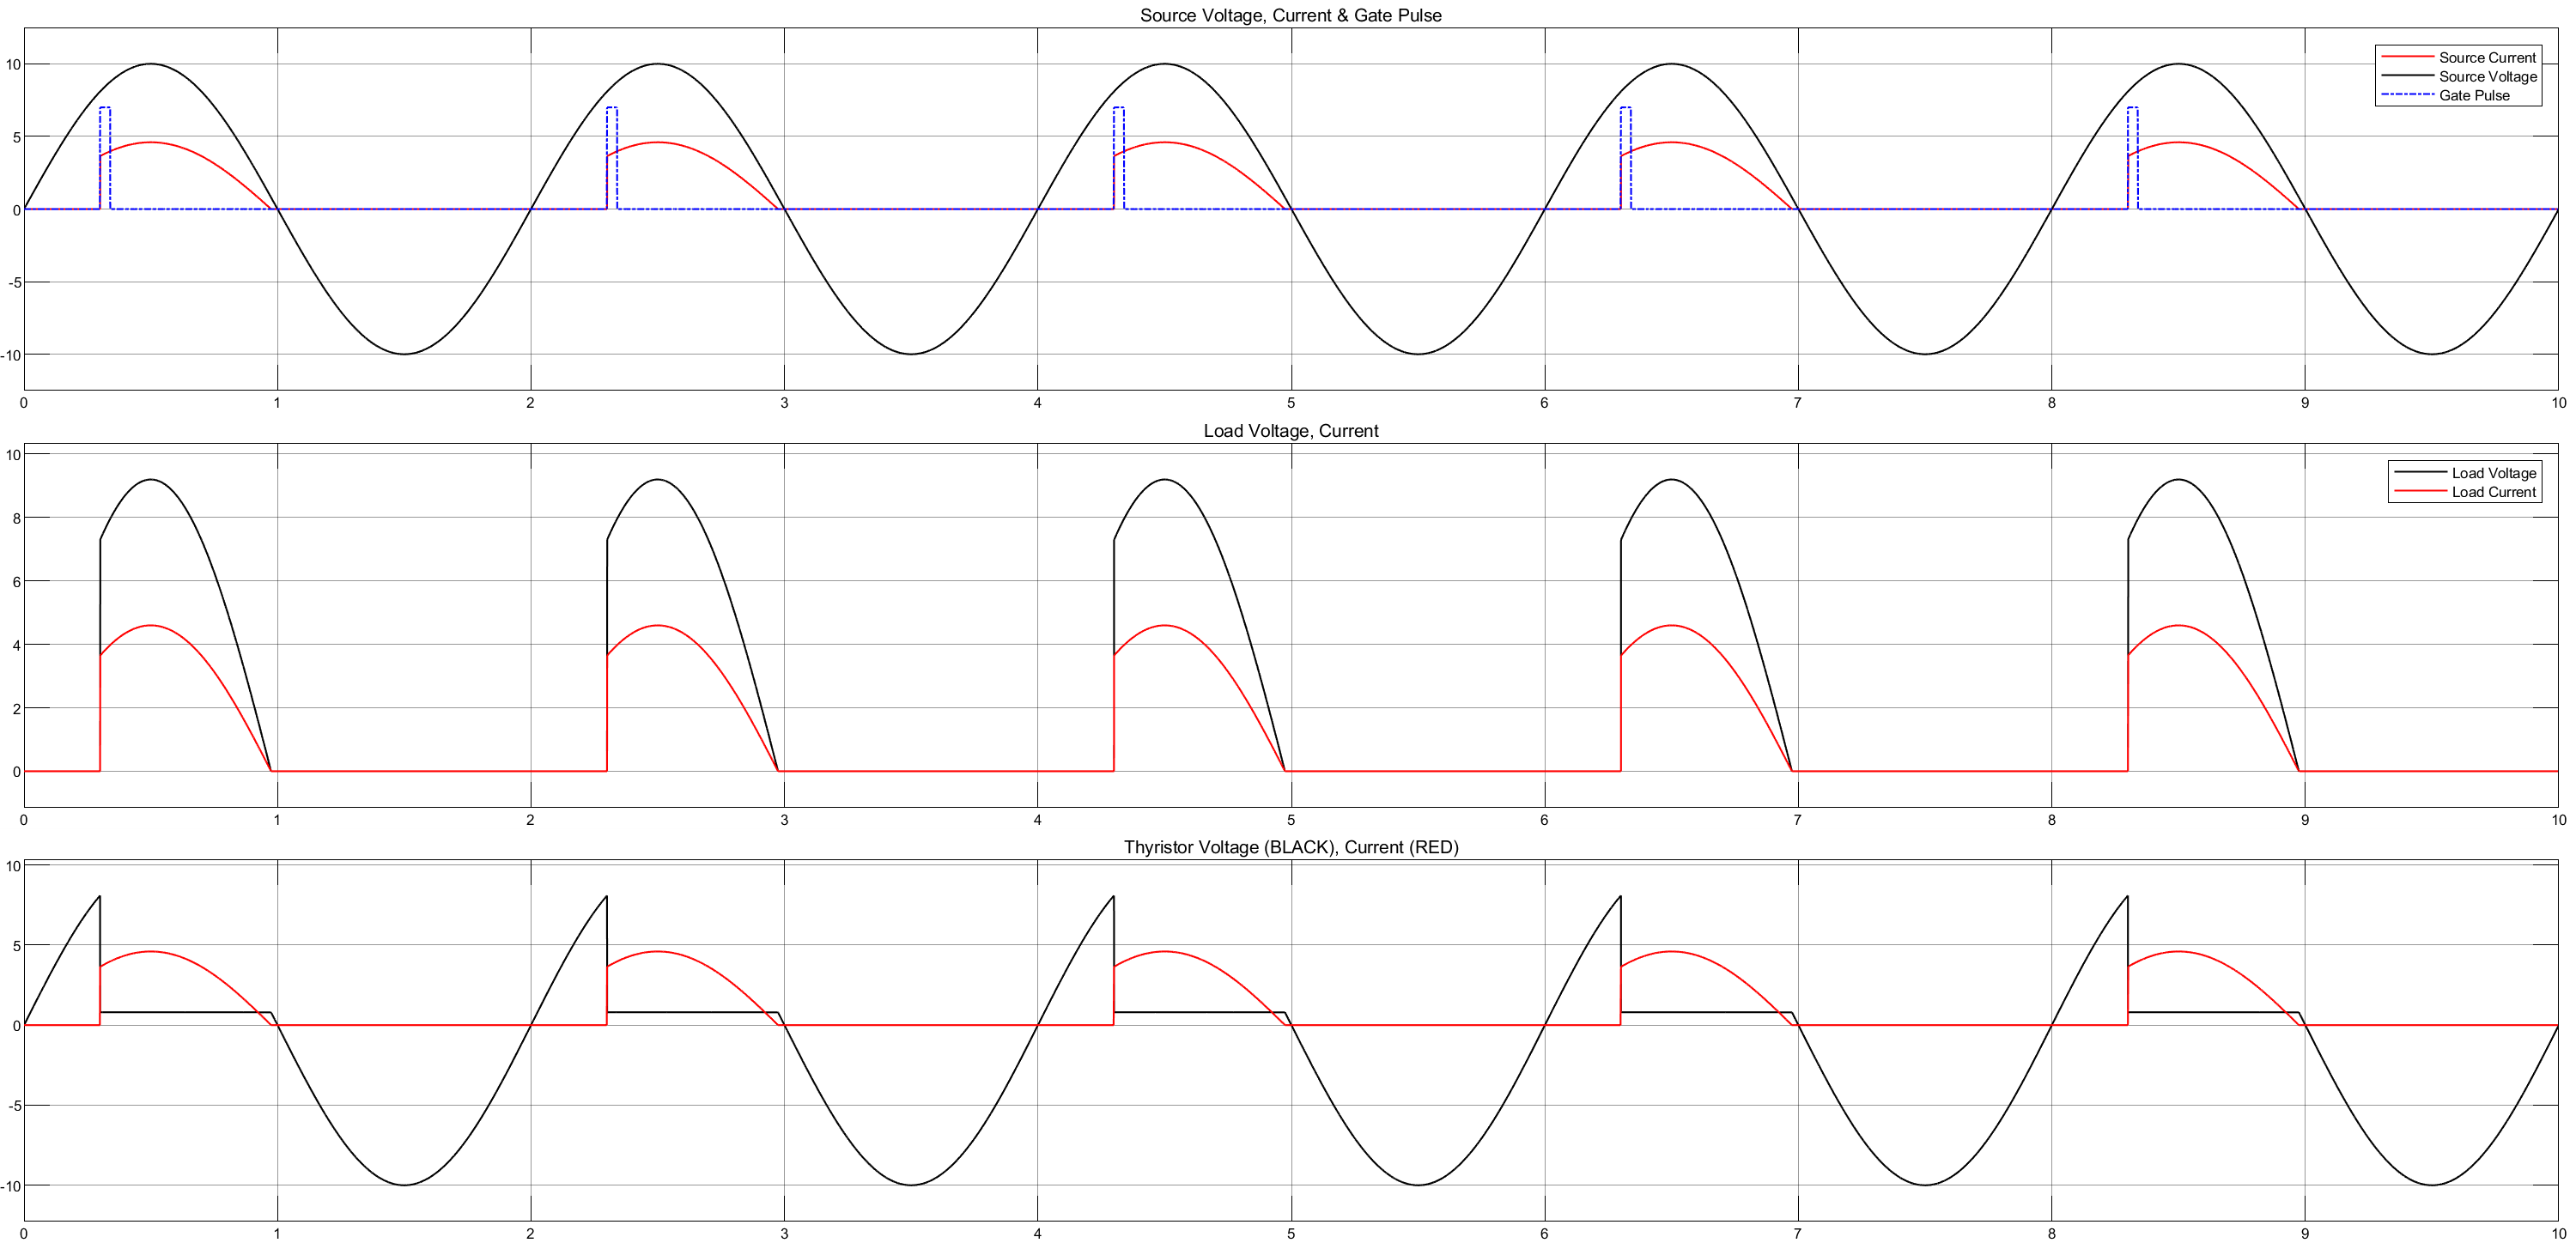
\includegraphics[width=\textwidth]{r_delay.png}
    \caption{Oscilloscope Output for R Load, With Gate Voltage Delay}
    \label{fig:rLoadDelay}
\end{figure}

\begin{figure}[H]
    \centering
    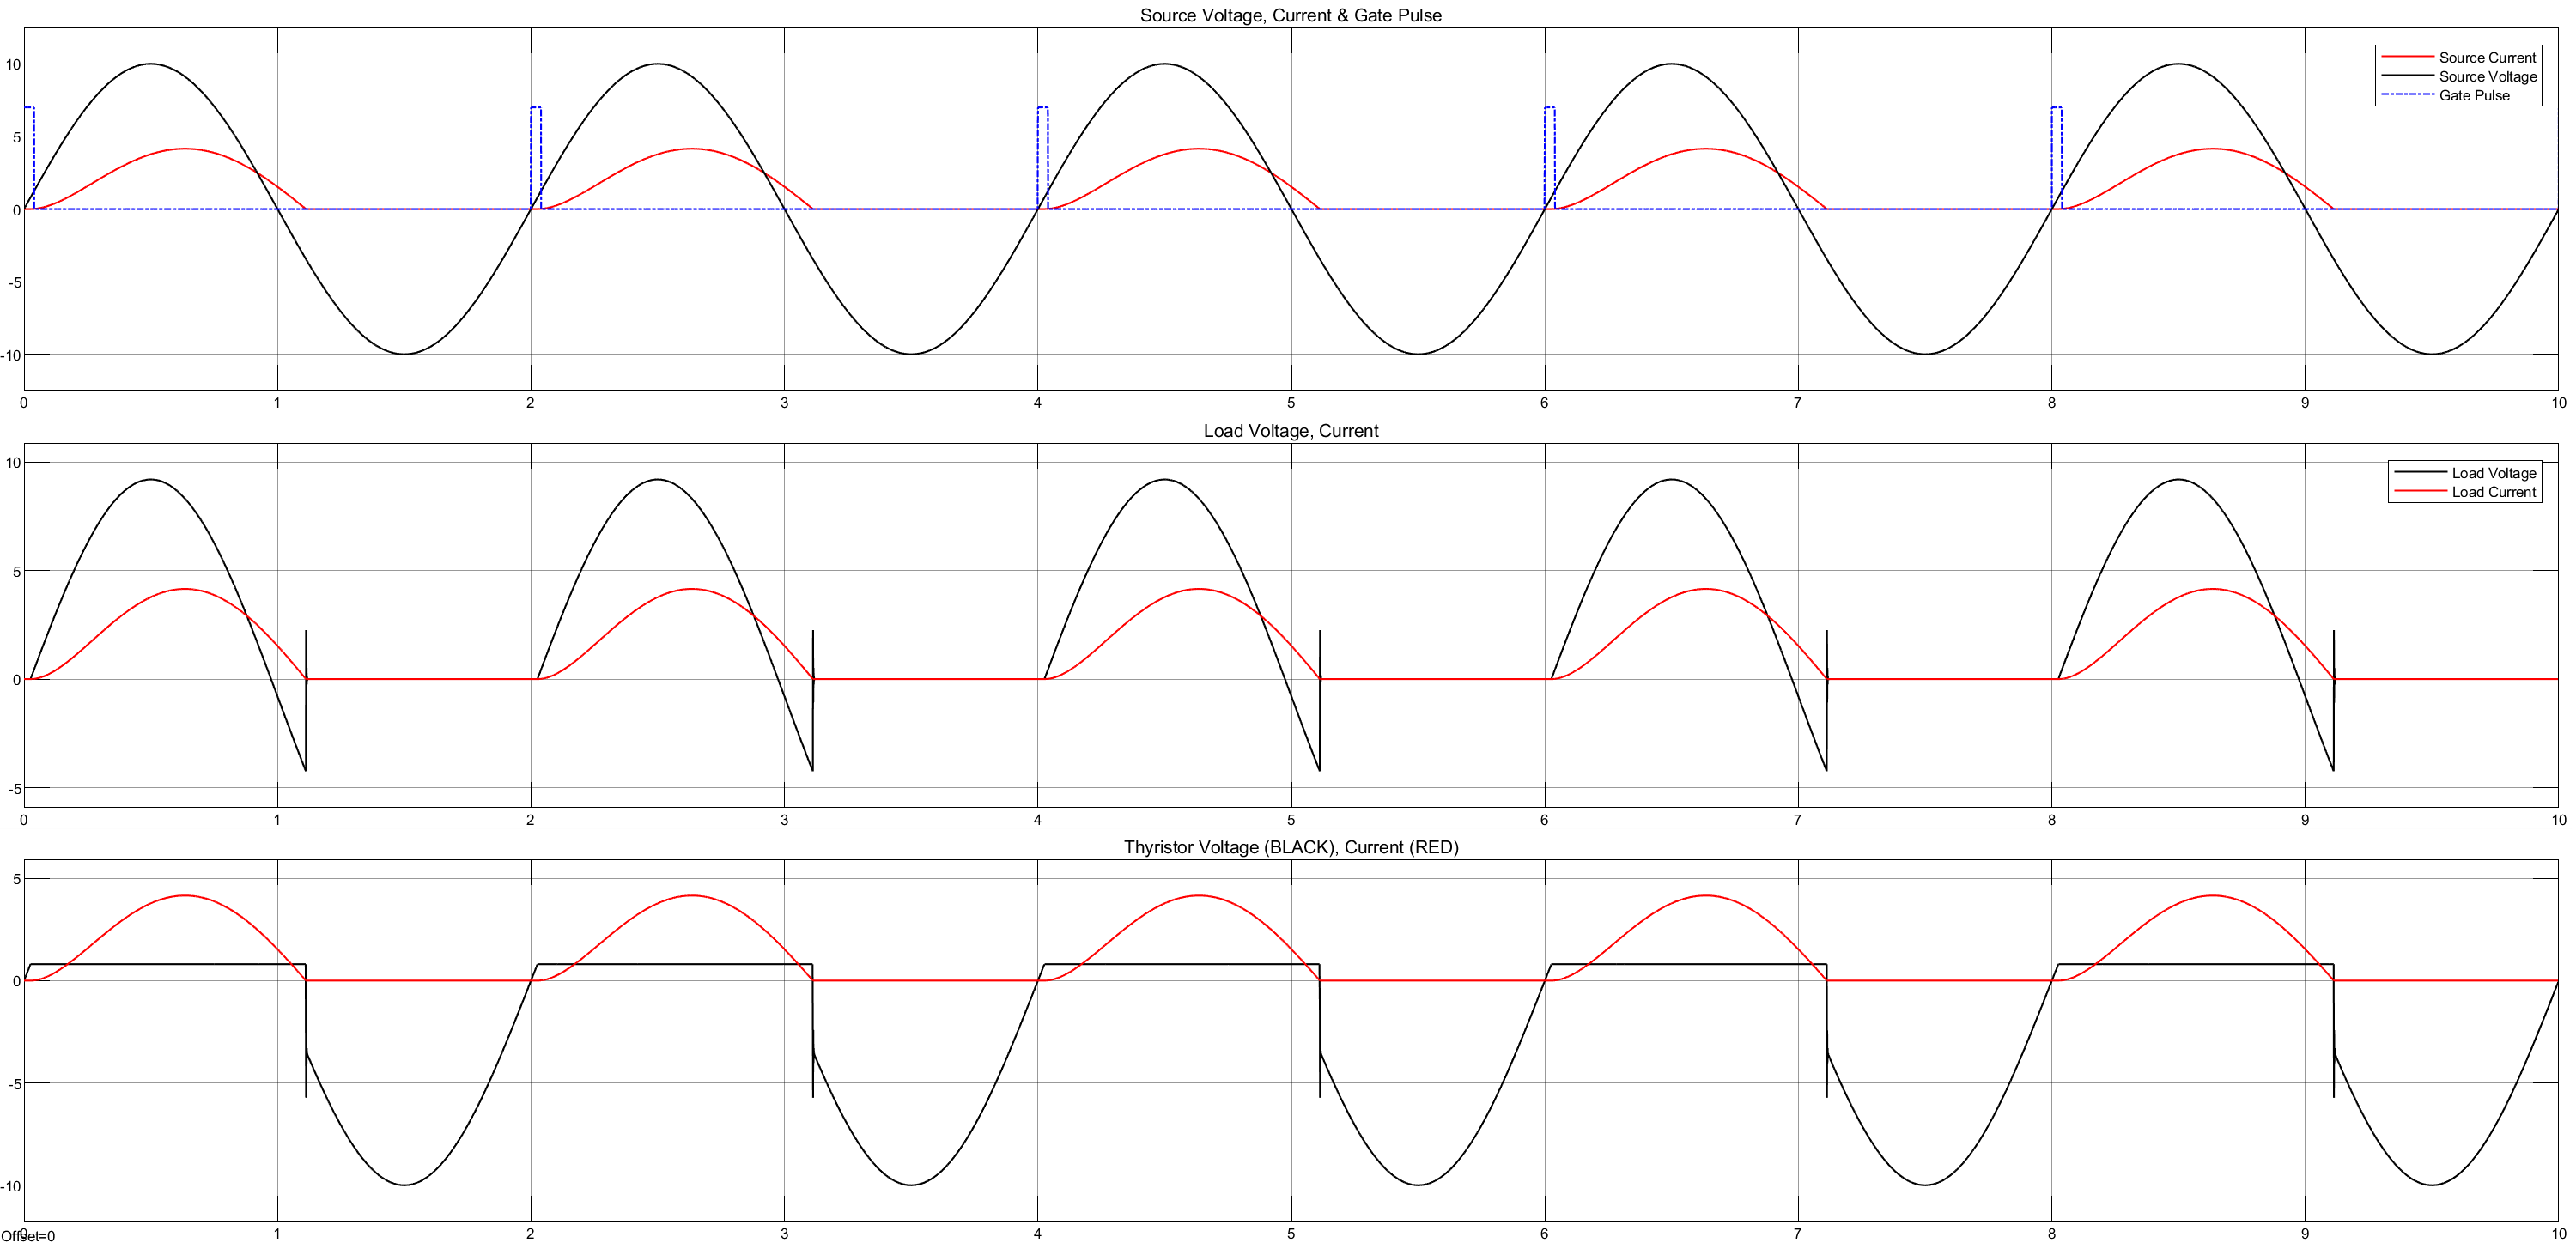
\includegraphics[width=\textwidth]{rl.png}
    \caption{Oscilloscope Output for RL Load, No Gate Voltage Delay}
    \label{fig:rlLoad}
\end{figure}

\begin{figure}[H]
    \centering
    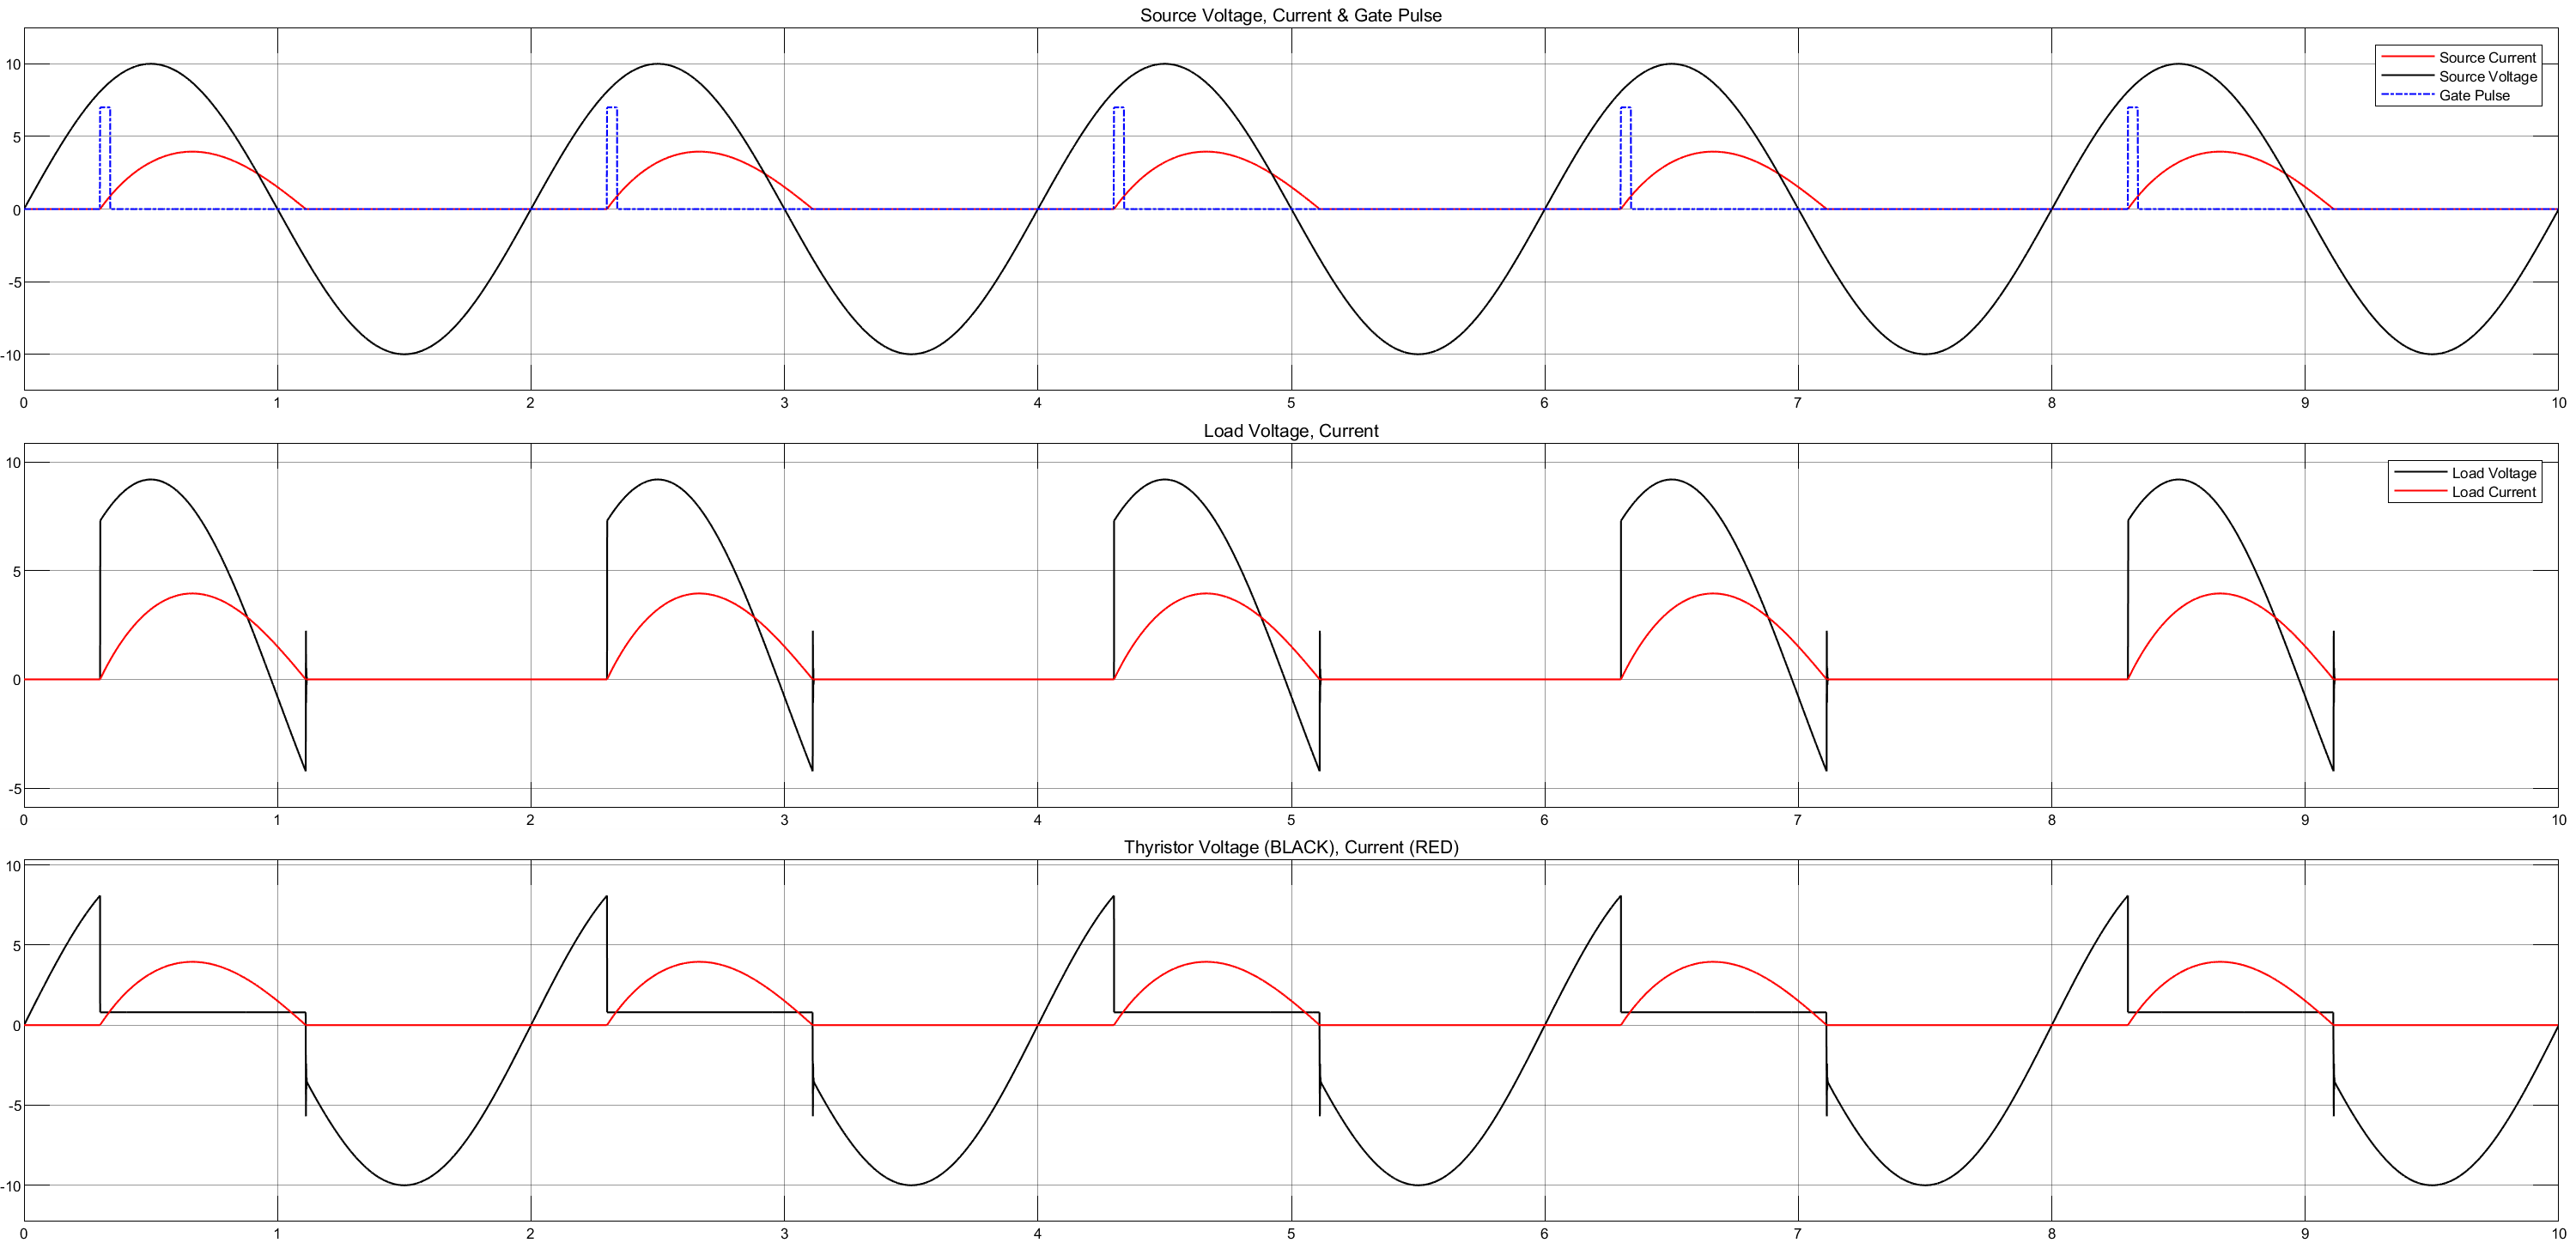
\includegraphics[width=\textwidth]{rl_delay.png}
    \caption{Oscilloscope Output for RL Load, With Gate Voltage Delay}
    \label{fig:rlLoadDelay}
\end{figure}

\section*{Discussion}
\addcontentsline{toc}{section}{Discussion}
The experiment explores the characteristics of a thyristor under different load conditions using DC and AC supplies. The thyristor's behavior in forward bias, reverse bias, and rectification is observed using simulation software. The oscilloscope and signal generator help analyze the thyristor's response to various input signals and load conditions. The experiment enhances understanding of the thyristor's operation and its applications in electronic circuits.

\section*{Conclusion}
\addcontentsline{toc}{section}{Conclusion}
The experiment investigates the characteristics of a thyristor under different load conditions using DC and AC supplies. The thyristor's behavior in forward bias, reverse bias, and rectification is observed using simulation software. The oscilloscope and signal generator help visualize the thyristor's response to various input signals and load conditions. The experiment enhances understanding of the thyristor's operation and its applications in electronic circuits.

\bibliographystyle{IEEEtran}
\renewcommand{\bibname}{References}
\addcontentsline{toc}{section}{References}
\bibliography{ref}

\end{document}
